\documentclass{article}
\usepackage[utf8]{inputenc}
\usepackage{tabularx} % extra features for tabular environment
\usepackage{amsmath}  % improve math presentation
\usepackage{graphicx} % takes care of graphic including machinery
\usepackage{xspace}
\usepackage{tikz}
\usepackage{enumitem}
\usetikzlibrary{babel}
\usepackage[american]{circuitikz}
\usetikzlibrary{calc}
\usepackage{siunitx}
\usepackage{pgfplots}
\usepackage[skins,theorems]{tcolorbox}
\tcbset{highlight math style={enhanced,
  colframe=red,colback=white,arc=0pt,boxrule=1pt}}
\pgfplotsset{width=10cm,compat=1.9}
\usepackage[margin=1in,letterpaper]{geometry} % decreases margins
\usepackage{float}
\usepackage{cite} % takes care of citations
\usepackage[final]{hyperref} % adds hyper links inside the generated PDF file
\hypersetup{
colorlinks=true,       % false: boxed links; true: colored links
linkcolor=blue,        % color of internal links
citecolor=blue,        % color of links to bibliography
filecolor=magenta,     % color of file links
urlcolor=blue        
}
\usepackage{listings}
\usepackage{xcolor}

\definecolor{codegreen}{rgb}{0,0.6,0}
\definecolor{codegray}{rgb}{0.5,0.5,0.5}
\definecolor{codepurple}{rgb}{0.58,0,0.82}
\definecolor{backcolour}{rgb}{1, 1, 1}

\lstdefinestyle{mystyle}{
    backgroundcolor=\color{backcolour},   
    commentstyle=\color{codegreen},
    keywordstyle=\color{magenta},
    numberstyle=\tiny\color{codegray},
    stringstyle=\color{codepurple},
    basicstyle=\ttfamily\footnotesize,
    breakatwhitespace=false,         
    breaklines=true,                 
    captionpos=b,                    
    keepspaces=true,                      
    showspaces=false,                
    showstringspaces=false,
    showtabs=false,                  
    tabsize=2
}

\lstset{style=mystyle}

\begin{document}

\title{{\textbf{PRML HOMEWORK 1}}}
\author{\textbf{TADIPATRI UDAY KIRAN REDDY}\\\textbf{EE19BTECH11038}}
\maketitle

\section*{\hfil HW-1}
Apply Newtons method to steepest-descent algorithm to the optimal step size $\eta$, and check how many iterations are required for convergence.
\begin{equation*}
\overline{w}^{new} = \overline{w}^{old} + \eta{\mathbf{X}^T(\mathbf{t}-\mathbf{X}\overline{w})}|_{\overline{w} = \overline{w}^{old}}
\end{equation*}
\newline
\newline
We find that optimal step size $\eta$ should be the inverse of Hessian matrix, $\left(\frac{{\partial}^2 J(\overline{w})}{\partial \overline{w} \partial \overline{w}^T}\right)^{-1} = \left(\textbf{X}^T\textbf{X}\right)^{-1}$.\\
Using substituting the optimal $\eta$ in update equation we get,\\
\textbf{\#Iteration = 1}
\begin{gather*}
\overline{w}^{new} = \overline{w}^{old} + \left(\textbf{X}^T\textbf{X}\right)^{-1}{\mathbf{X}^T(\mathbf{t}-\mathbf{X}\overline{w})}|_{\overline{w} = \overline{w}^{old}}\\
\implies \overline{w}^{new} = \left(\textbf{I} - \left(\textbf{X}^T\textbf{X}\right)^{-1}\textbf{X}^T\textbf{X}\right){\overline{w}_{old}} + \left(\textbf{X}^T\textbf{X}\right)^{-1}{\mathbf{X}^T\mathbf{t}}\\
\implies \overline{w}_{new} = w^{*}
\end{gather*}
So theoritically only one iteration is sufficient with optimal eta to make the solution to converge to optimal weights.\\
The implementation of this algorithm is given here Appendix \ref{code:hw1}. The data generated here is just the equation
\begin{equation*}
	t = 3.879x - 65
\end{equation*}
\begin{figure}[H]
	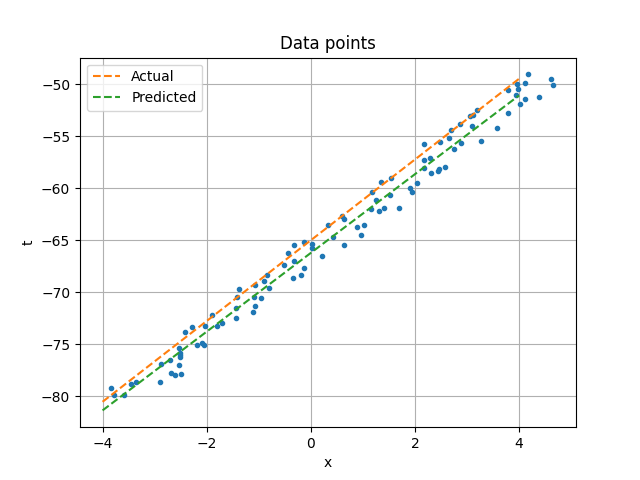
\includegraphics[scale=0.5]{./figs/datapoints.png}
	\caption{Data points}
	\label{fig:dp}
\end{figure}
\begin{figure}[H]
	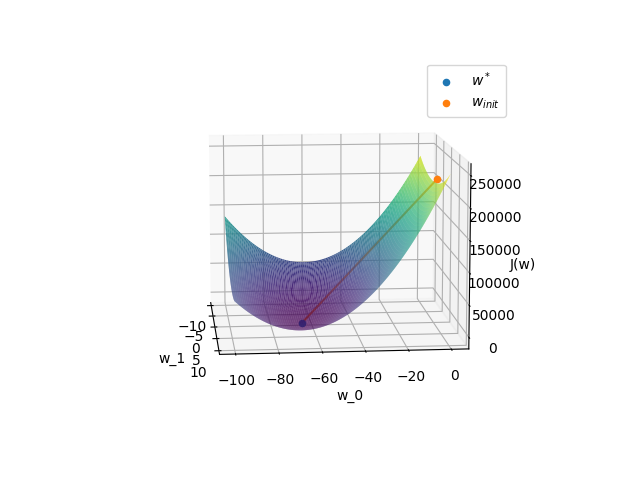
\includegraphics[scale=1]{./figs/3d.png}
	\caption{Error surface with path of steepest descent algorithm.}
	\label{fig:error}
\end{figure}
Observe that in Figure \ref{fig:error}, it took only 1 iteration to converge to the desired solution, this has been proved mathematically as well.
\begin{figure}[H]
	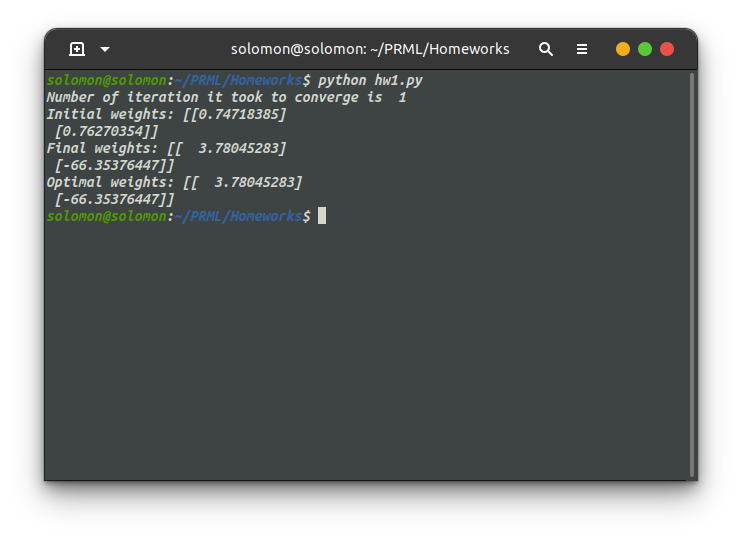
\includegraphics[scale=0.38]{./figs/op.png}
	\caption{Output}
	\label{fig:op}
\end{figure}
\section*{\hfil HW-2}
Suppose you are experimenting with L1 and L2 regularization. Further imagine that you are running gradient descent and at some iteration your weight vector is $\overline{w}$ = [1, $\epsilon$] $\in$ $R^2$ where $\epsilon > 0$ is very small. With the help of this example explain why L2 norm does not encourage sparsity i.e., it will not try to drive $\epsilon$ to 0 to produce a sparse weight vector. Give mathematical explanation.
\newline
\newline

%Let after GDA we observe that change in weight vector is $\Delta \overline{w} = \begin{bmatrix}\Delta w_1 & \Delta w_2 \end{bmatrix} ^T$. Then $\overline{w} = \begin{bmatrix} 1-\Delta w_1 & \epsilon-\Delta w_2 \end{bmatrix} ^T$
%Take Case (i) where $\Delta w_1 > \Delta w_2$,\\
%\begin{gather*}
%J_{L1_{(i)}}(\overline{w}) = J(\overline{w}) + \lambda \left(1- \Delta w_1 + \epsilon - \Delta w_2\right)\\
%J_{L2_{(i)}}(\overline{w}) = J(\overline{w}) + \lambda \left(1 - 2{\Delta w_1} + (\Delta w_1)^2 + {\epsilon}^2 - 2{\epsilon \Delta w_2} + (\Delta w_2)^2\right)
%\end{gather*}
%Another case (i) where $\Delta w_1 < \Delta w_2$,\\
Since $\overline{w} = \begin{bmatrix} 1 & \epsilon \end{bmatrix}^T$ and $\epsilon > 0$.\\
\begin{gather*}
L_1(\overline{w}) = ||\overline{w}||_1 \implies \frac{\delta L_1{\overline{w}}}{\delta \overline{w}} = \begin{bmatrix} sgn(w_1) & sgn(w_2) \end{bmatrix} = \begin{bmatrix} 1 & 1 \end{bmatrix}\\
L_2(\overline{w}) = \frac{1}{2}||\overline{w}||^{2}_{2} \implies \frac{\delta L_2{\overline{w}}}{\delta \overline{w}} = \overline{w}^T
\end{gather*}
By applying GDA on this we get, for brevity we are ignoring the MSE cost since it is a common term for both
\begin{gather*}
\overline{w}_{L1} = \begin{bmatrix}
1 - {\eta}{\lambda} \\
\epsilon - {\eta}{\lambda}
\end{bmatrix}\\
\overline{w}_{L2} = (1 - {\eta}{\lambda}) \begin{bmatrix}
1 \\
\epsilon
\end{bmatrix}
\end{gather*}
Since $\epsilon$ is very small and it is most likely to tend to zero than 1 in L1 regulatisation but where as in the case of L2 we see that both dimensions are equally scaled and also it's gradient depends upon current weights. In L1 even if second diemension is negative the gradients are -1 and it tries to bring it to zero. But in the case L2 it just scale down the weights.\\
 Thus we can say that L2 norm does'nt encourage sparsity compared to L1.
\section*{\hfil HW-3}
Till now we have been considering a scalar target t from a vector of input observations $\overline{x}$. How do you extend this approach for regressing a vector of targets $\overline{t} = (t1, t2, ..., tp)$. Derive the close form solutions and write sequential update equations using SGD.
\begin{table}[H]
\begin{tabular}{||c|c||}
\hline
Variable & Dimension \\
\hline
$\mathbf{T}$ & N X P \\
\hline
$\mathbf{X}$ & N X (D+1) \\
\hline
$\mathbf{W}$ & (D+1) X P \\
\hline
$\mathbf{E}$ & N X P\\
\hline
\end{tabular}
\end{table}

Where N is number of examples, P is output vector dimension and D is input vector dimension.\\
\newline 
Taking our cost function as Forbenious norm(Appendix \ref{eq:fn}) of Error Matrix($\mathbf{E}$).
\begin{gather*}
\mathbf{E} = \mathbf{T} - \mathbf{XW}\\
\tcbhighmath[drop fuzzy shadow]{J(\mathbf{W}) = \frac{1}{2}||\mathbf{E}||^2_{F}}
\end{gather*}
We obtain optimal weights by differentiating and equation to zero.
\begin{gather*}
\frac{\partial J(\mathbf{W})}{\partial \mathbf{W}} = -\mathbf{X}^T\left(\mathbf{T} - \mathbf{XW}\right) = 0\\
\implies \tcbhighmath[drop fuzzy shadow]{\mathbf{W}^* = (\mathbf{X}^T\mathbf{X})^{-1}\mathbf{X}^T\mathbf{T}}
\end{gather*}
Now we obtain stochastic gradient descent equations,
\begin{gather*}
\mathbf{W}_{(n+1)} = \mathbf{W}_{(n)} - \mathbf{\eta}\frac{\partial J(\mathbf{W})}{\partial \mathbf{W}}\\
\tcbhighmath[drop fuzzy shadow]{\mathbf{W}_{(n+1)} = \mathbf{W}_{(n)} + \mathbf{\eta}\mathbf{X}^T\left(\mathbf{T} - \mathbf{XW}\right)}
\end{gather*}
Using taylor series we find optimal $\eta$,
\begin{gather*}
J(\mathbf{W} + \Delta \mathbf{W}) = J(\mathbf{W}) + \Delta \mathbf{W}^T {\nabla}J(\mathbf{W}) + \frac{1}{2} \Delta \mathbf{W}^T {\nabla}^2J(\mathbf{W})\Delta \mathbf{W}\\
\frac{\partial J(\mathbf{W} + \Delta \mathbf{W})}{\partial \Delta \mathbf{W}} = \mathbf{0} = {\nabla}J(\mathbf{W}) + {\nabla}^2J(\mathbf{W})\Delta \mathbf{W} \\
\implies \tcbhighmath[drop fuzzy shadow]{\Delta \mathbf{W}^* = -({\nabla}^2J(\mathbf{W}))^2{\nabla}J(\mathbf{W})}\\
\implies \tcbhighmath[drop fuzzy shadow]{{\eta}^* = (\mathbf{X}^T\mathbf{X})^{-1}}
\end{gather*}
\section*{\hfil Appendix}

\subsection*{HW1 implementation}
\begin{lstlisting}[caption={Python implementation of steepest decent algorithm with optimal $\eta$} ,language=python, label={code:hw1}] 
import numpy as np
import matplotlib.pyplot as plt

# Random linear data
def gen_data(N):
	X = np.linspace(-4, 4, N)
	X = X.reshape(N, 1)
	t = 3.879*X - 65
	t = t + np.random.rand(N, 1)
	X = X + np.random.rand(N, 1)
	return t, X

# J(w)
def cost(t, X, w):
	e = t - X@w
	return 0.5*e.T@e

N = 100

t, X_data = gen_data(N)

ones = np.ones((N, 1))
X = np.hstack((X_data, ones))

w = np.random.rand(2, 1)
w_init = w


# GDA
def steepest_decent(t, X, w, eta):
	# print(w.shape, (X.T@(t-X@w)).shape)
	if type(eta) is np.ndarray:
		return w + eta@(X.T@(t-X@w))
	else:
		return w + eta*(X.T@(t-X@w))

tolerance = 1e-6
def converged(w_old, w_new, tolerance):
	x = np.linalg.norm(w_old-w_new)/np.linalg.norm(w_old)
	return x <= tolerance

itr = 0

eta = np.linalg.inv(X.T@X)

err_data = []
err_data.append(np.array(([w[0, 0], w[1, 0], cost(t, X, w)[0, 0]])))

w_star = np.linalg.inv(X.T@X)@(X.T)@t



while not converged(w, w_star, tolerance):
	w = steepest_decent(t, X, w, eta)
	itr += 1
	err_data.append(np.array(([w[0, 0], w[1, 0], cost(t, X, w)[0, 0]])))

err_data = np.array(err_data).T

print("Number of iteration it took to converge is ", itr)
print("Initial weights: {}".format(w_init))
print("Final weights: {}".format(w))
print("Optimal weights: {}".format(w_star))

w_1 = np.linspace(-10, 10, 100)
w_0 = np.linspace(-100, 0, 100)

XX, YY = np.meshgrid(w_1, w_0)

ZZ = np.empty_like(XX)

for i in range(XX.shape[0]):
	for j in range(XX.shape[1]):
		w_ = np.array([XX[i, j], YY[i, j]]).reshape(2, 1)	
		e_ = t - X@w_
		ZZ[i, j] = 0.5*e_.T@e_

plt.figure()
plt.title("Data points")
plt.plot(X_data[:, 0], t[:, 0], ".")
plt.plot(np.linspace(-4, 4, 100), 3.879*np.linspace(-4, 4, 100) - 65, "--", label="Actual")
plt.plot(np.linspace(-4, 4, 100), w[0, 0]*np.linspace(-4, 4, 100) + w[1, 0], "--", label="Predicted")
plt.grid()
plt.legend()
plt.xlabel("x")
plt.ylabel("t")

fig = plt.figure()
ax = plt.axes(projection='3d')
ax.plot_surface(XX, YY, ZZ, rstride=1, cstride=1, cmap='viridis', edgecolor='none')
ax.plot(err_data[0, :], err_data[1, :], err_data[2, :])
ax.scatter(w_star[0, 0], w_star[1, 0], cost(t, X, w_star)[0, 0], label=r'$w^*$')
ax.scatter(w_init[0, 0], w_init[1, 0], cost(t, X, w_init)[0, 0], label=r'$w_{init}$')
ax.set_xlabel('w_1')
ax.set_ylabel('w_0')
ax.set_zlabel('J(w)');
ax.legend()
plt.show()
\end{lstlisting}

\subsection*{Frobenius norm}
\begin{equation} \label{eq:fn}
	||\mathbf{A}||_{F} = \sqrt{\sum_{i=1}^N\sum_{j=1}^{M}A^2_{ij}}
\end{equation}
\end{document}